\section {Protocole Expériment}


\subsection{Matériel utilisé}

Le design de l'architecture sert à décider comment définir les unités de traitement et la communication entre elles. La définition des unités de traitement suit le découpage du pipeline de reconnaissance avec des nœuds responsables pour la segmentation, calcul de features et la classification, aussi comme, le contrôle du robot.

L'interfaçage matériaux-logiciel était fait sur l'environnement ROS -
Robot Operating System. Aussi que les outils d'affichage, ROS, 
rassemble les librairies d'acquisition d'images RGB-D, OpenNi 2 et Freenect, et de traitement de nuage de point, PCL.
De même, sa structure de nœuds a permis une implémentation modulaire et direct du
système décrit au-dessus, bien comme la communication entre machines, l'ordinateur portable et celui embarqué au robot.

L'image *10* illustre l'architecture en soulignant le flux d'information à travers des nœuds.

\subsection{Setup expérimental}
D'abord, vingt objets de tailles et formes diverses ont été choisi pour évaluer les capacités *récognitif* du robot. Ils sont objets typiques qui peuvent être faciliment retrouvés dans un laboratoire. Une liste avec tous est incorporé aux annexes. Ensuite, le feature VFH était calculé pour huit positions différents écartées de 45 dégréés. La position correspondent au angle zero, était choisi de manière aléatoire en alignant un des axes de l'objet avec celui du capteur. 

\begin{figure}[H]
	\subfloat{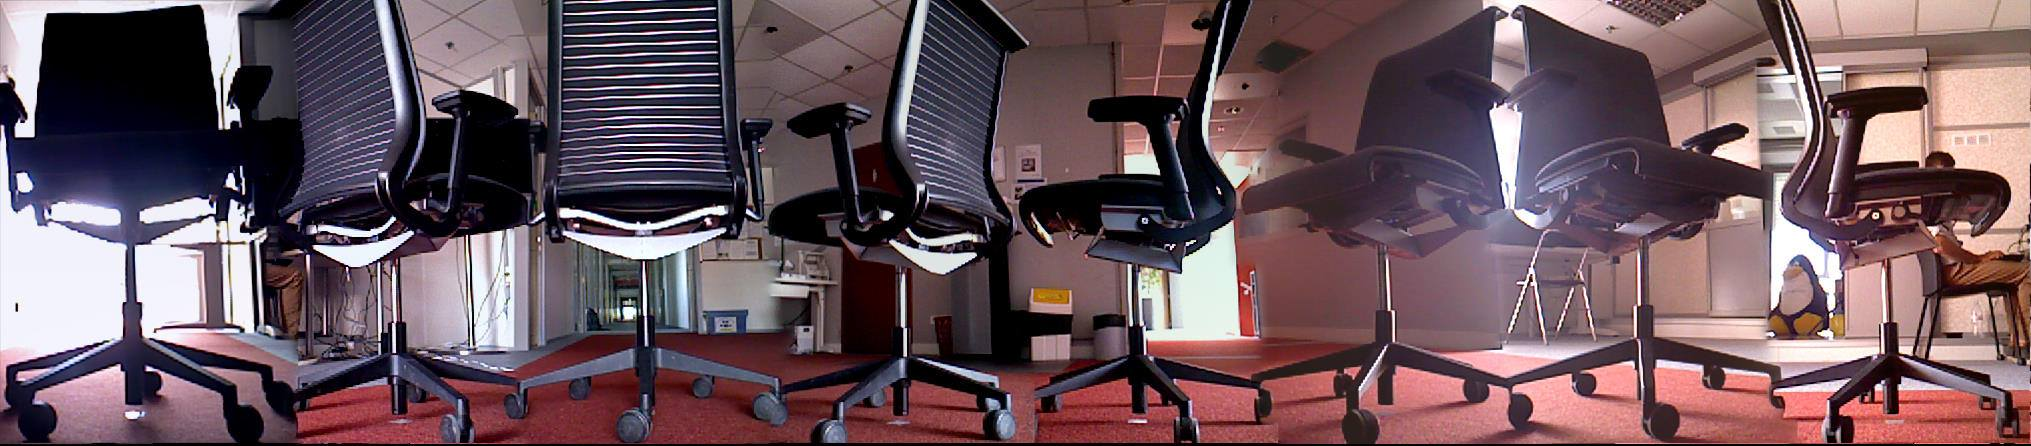
\includegraphics[width=\textwidth]{chair_db.jpg}}		
\end{figure}

\subsection {Création de la base de données}
Une première évaluation proposée consiste à faire un tour complèt autour de l'objet à être reconnu en quatre positions angulaires différentes : $0, 45, 90$ et une dernière choisi de manière aléatoire pour chaque objet. Le robot fait le tour à une vitesse de $0.35 \pm 0.1 m/s$ à une distance de $1.5m$, en enregistrant des images à $1hz$, ansi, une expérience typique consiste d'environ $25$  images d'angle différent et prendre $25 \pm 3$ seconds. Ensuite, trois différentes ratios sont calculés pour exprimer la reconnaissance d'objets, la reconnaissance de vue et la suivi des reconnaissances par la chaîne de Markov cachée.

\subsection{Résultats expérimentaux}

Un expérience typique est illustrée dans l'image {\color{green} ref} :

\begin{figure}[H]
	\subfloat{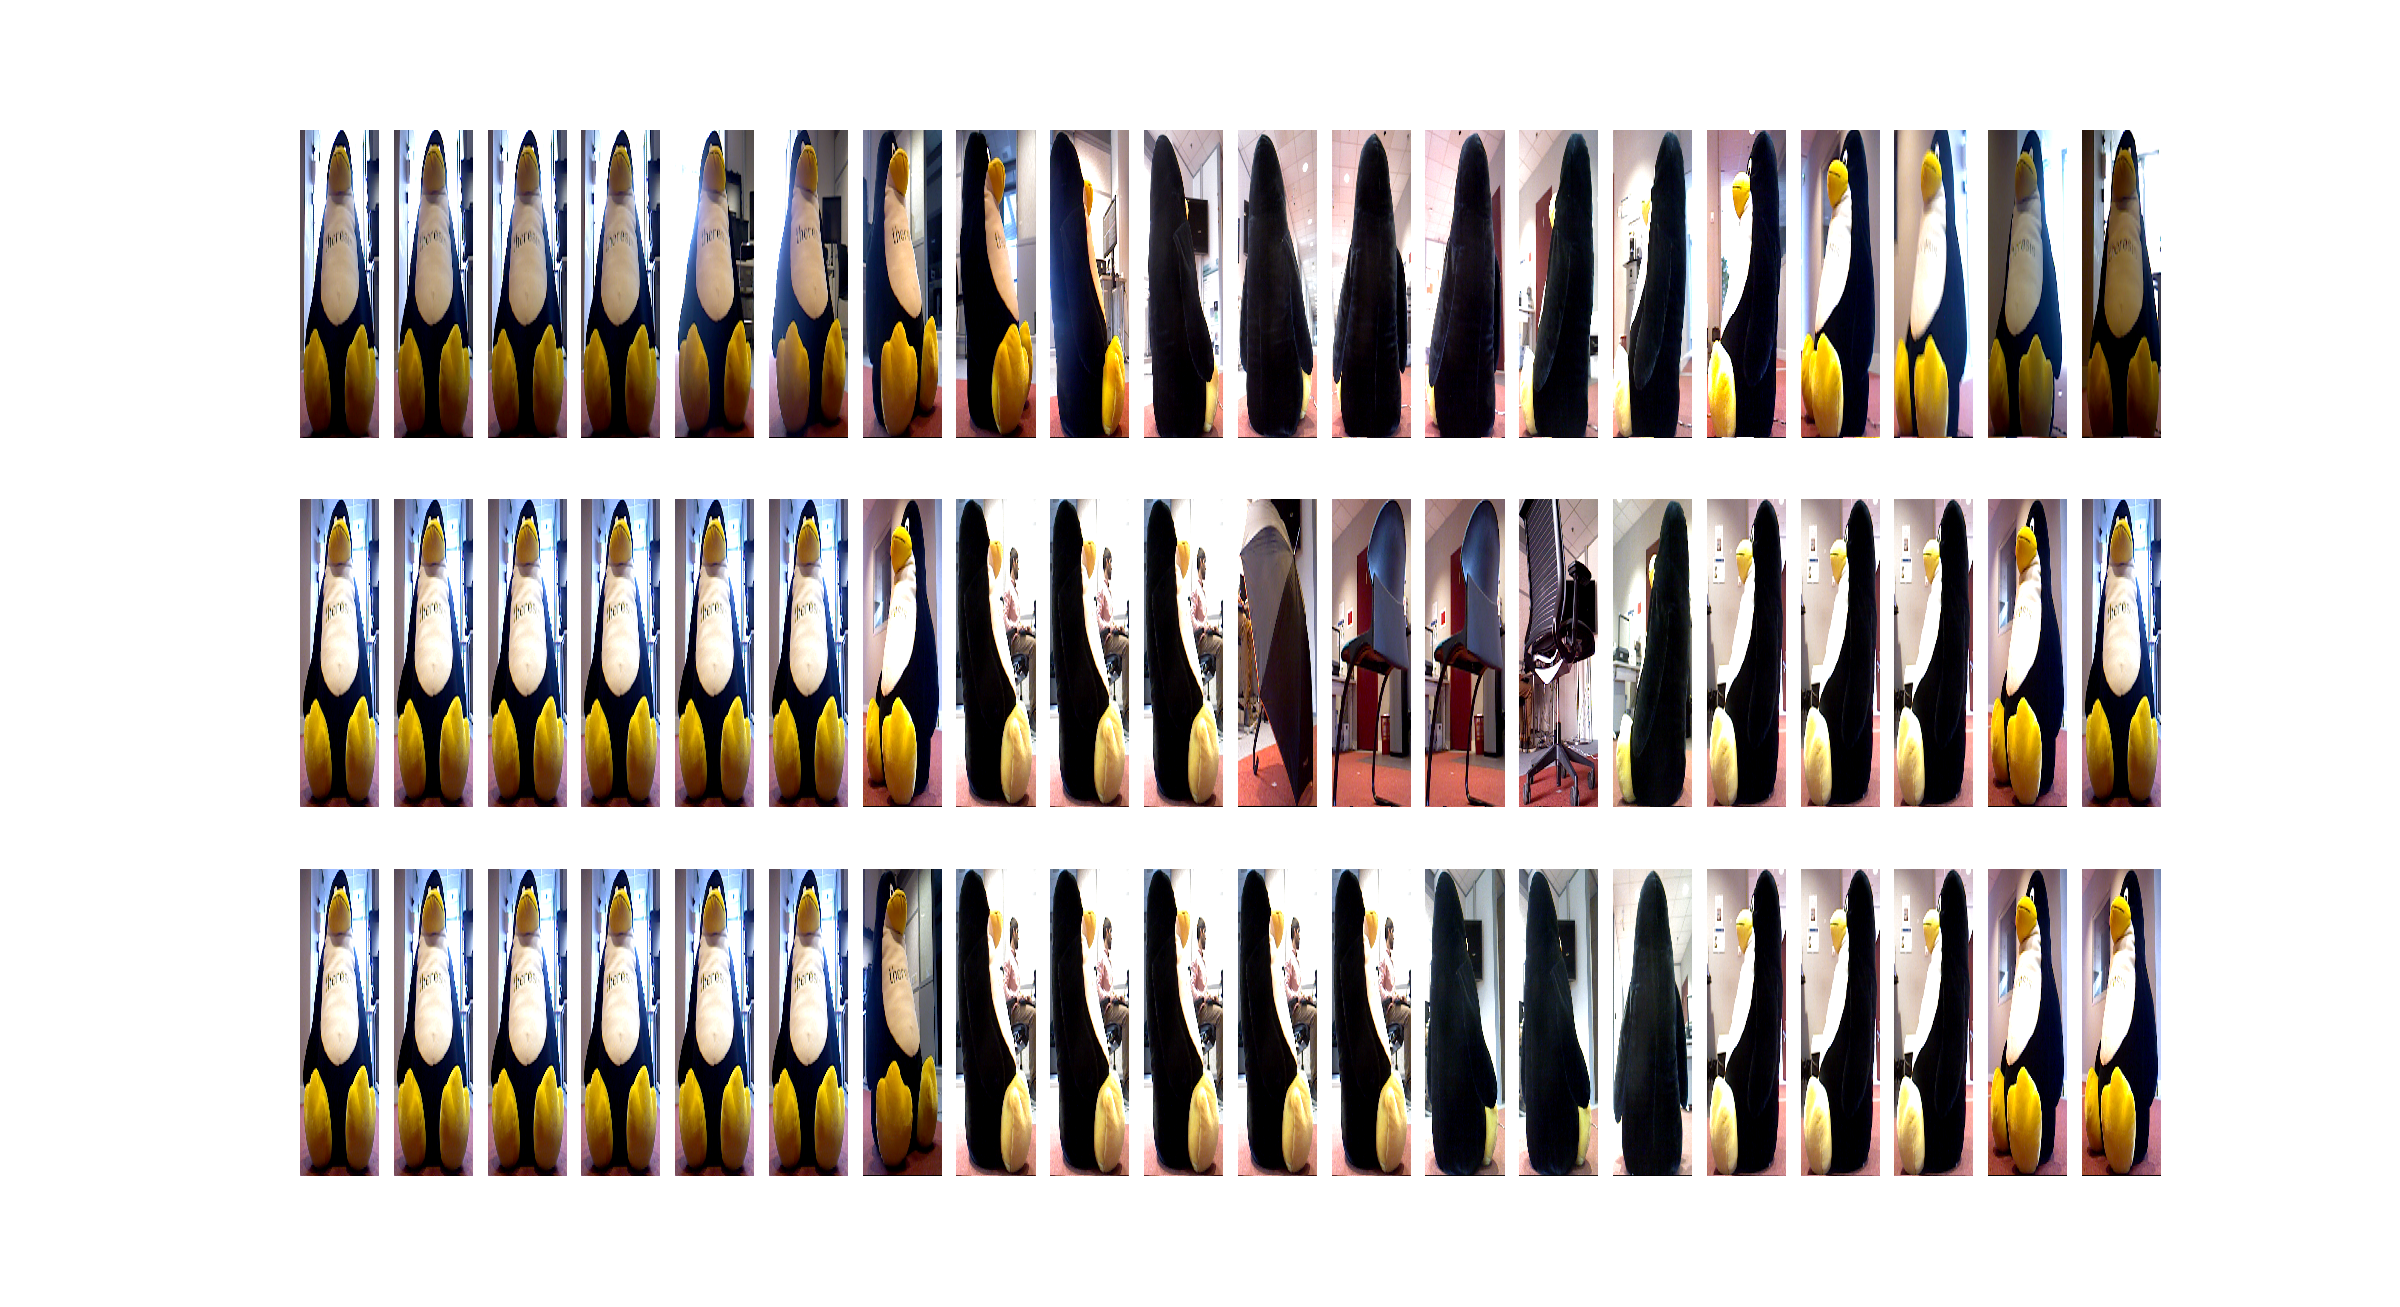
\includegraphics[width=\textwidth]{hmm_example.png}}		
\end{figure}

La première ligne correspond à l'image vue par le robot à chaque instant de temps et, donc, l'objet à être reconnu. Pendent que la deuxième, donnée par l'algorithme de reconnaissance, équivaut à la vue plus probable de l'objet reconnu par le K-plus proches voisins. Il est intéressant remarquer que l'invariance à rotation trompe l'estimation de l'orientation en prenant son correspond énantiomorphe dans le premier carré rouge. Autrement, la définition de murs enlève une grande partie du dos du pingouin dans l'étape de segmentation, ainsi, la définition de ce point de vu n'est pas suffisamment précis pour être différentié des autres objets, ce qui résulte dans une mauvaise reconnaissance dans le carré bleu. Au total, on remarque que le traitement fait par la chaîne de Markov cachée, surpasse les problèmes d'une base de donnée relativement sparse avec des possibles erreus de segmentation, pour atteindre la correction simultanée de la reconnaissance et de l'orientation. 

cela correspond à avoir une base

Finalement,  est affichée

\begin{figure}[H]
	\subfloat{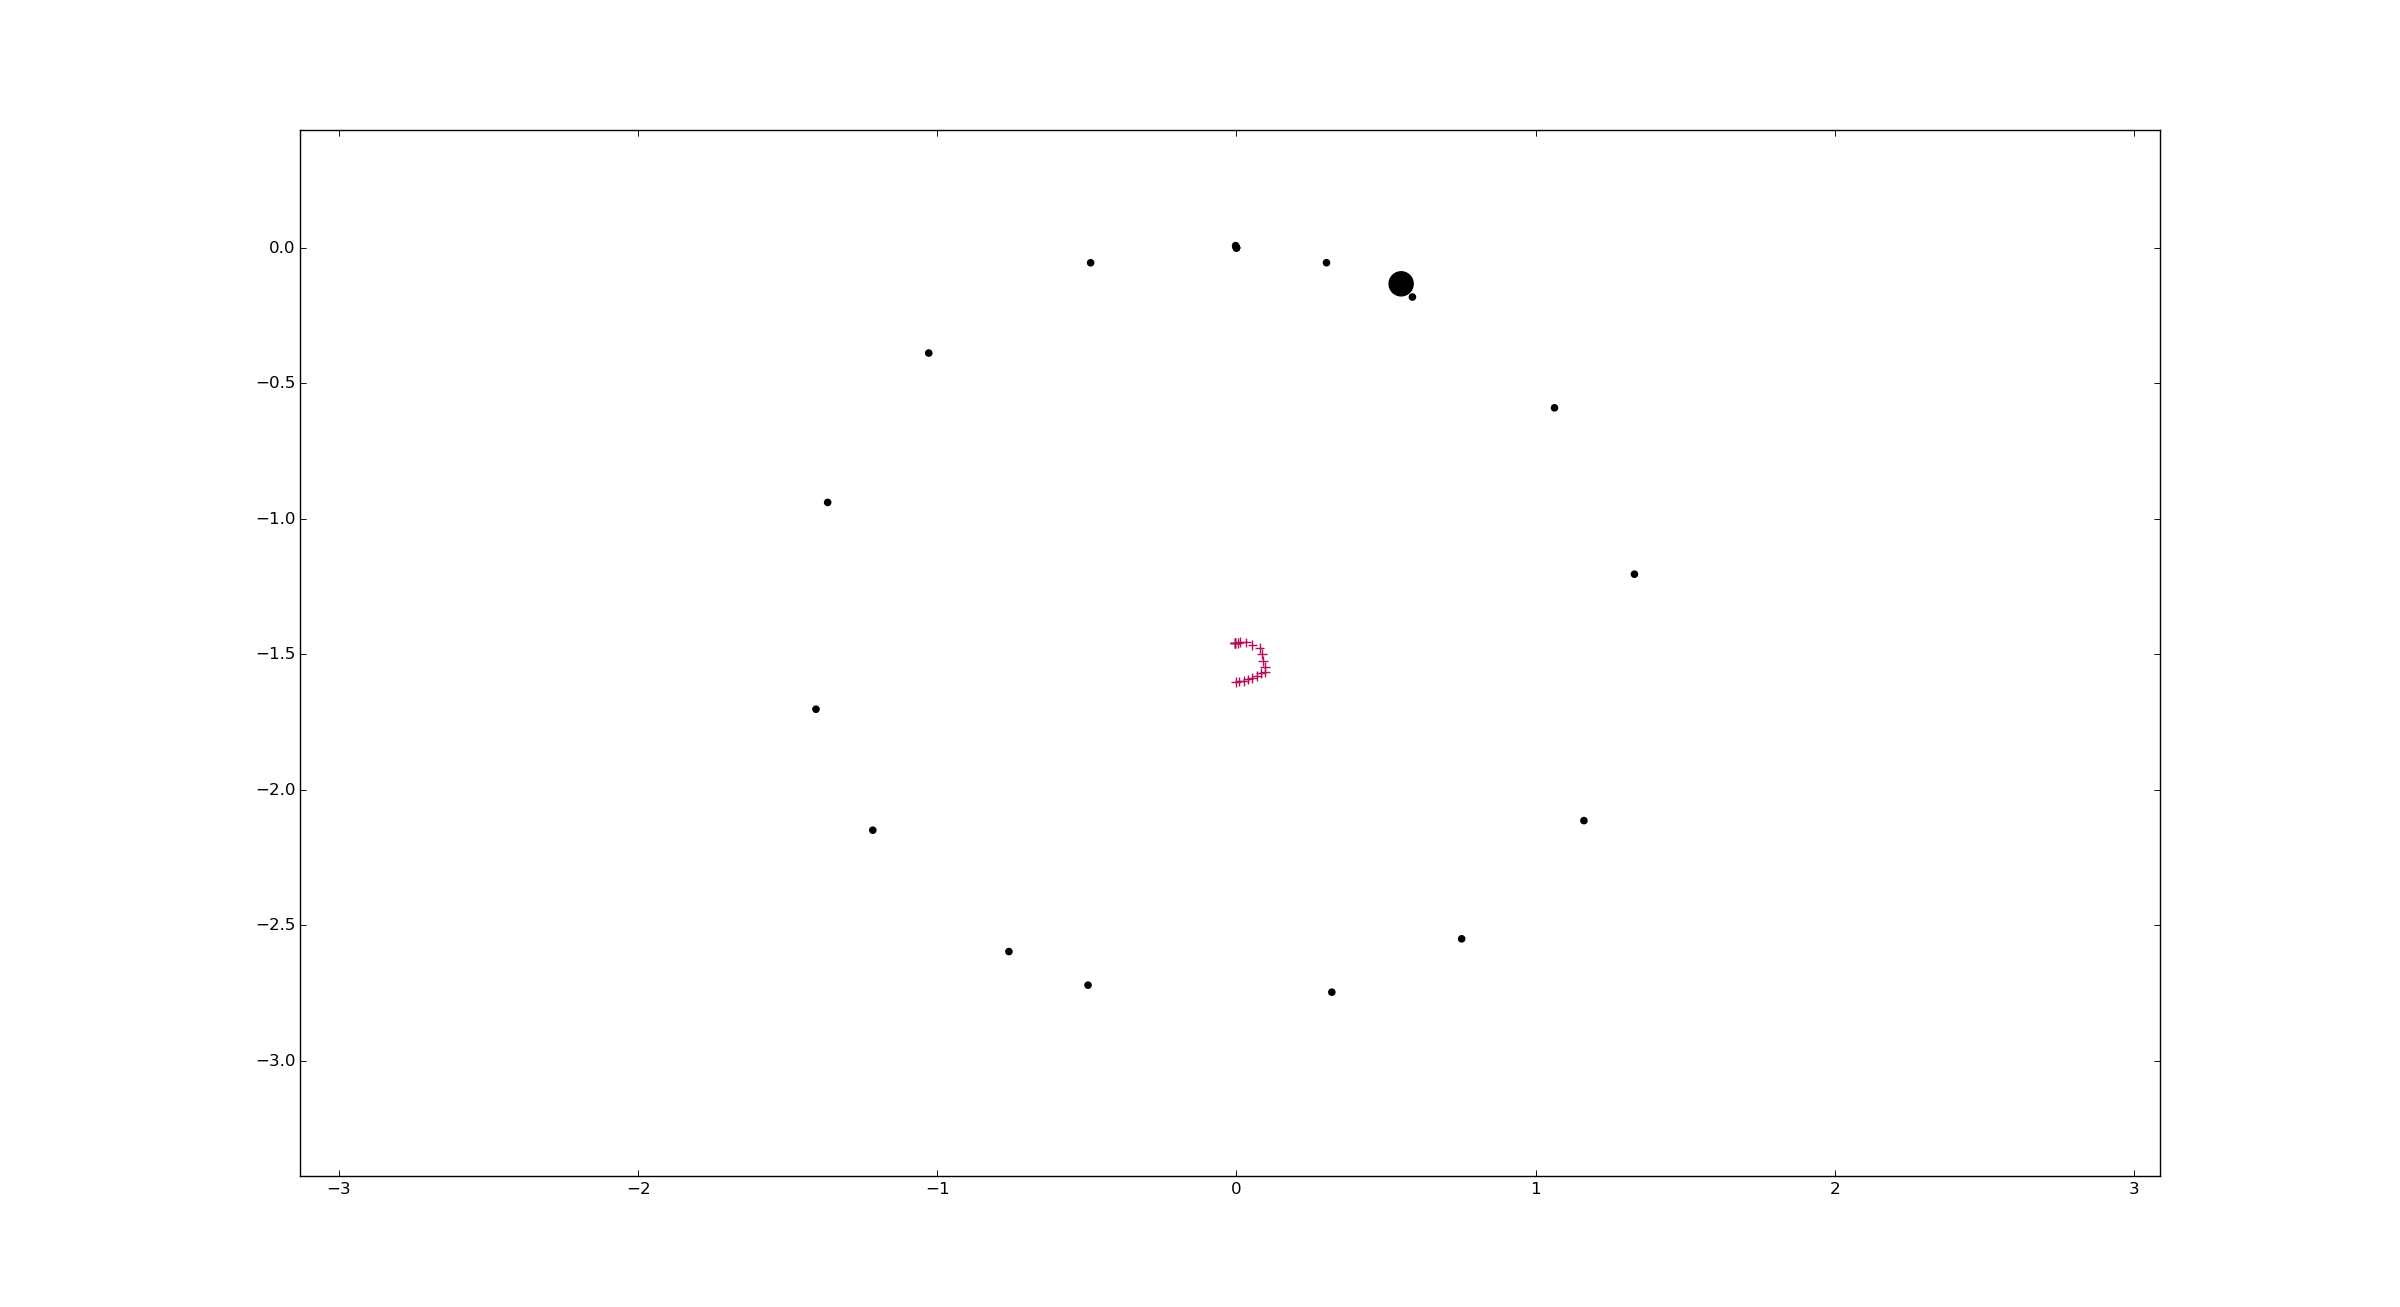
\includegraphics[width=\textwidth]{hmm_mov.png}}		
\end{figure}


{\color{green}
Dans le premier tableaux on retrouve le résultats de la reconnaissance donné par la comparaison des histogrammes provenant du *plus proche voisin*. Ce résultat estime la capacité de distinguer deux objets quelconques, en autre mots, cette capacité viens de la représentativité des descripteurs utilisés et l'efficacité de la mesure de similarité entre histogrammes.
}
